\title{Midterm I}
\author{
  Ethan Rooney
}
\date{\today}

\documentclass[12pt]{article}
\usepackage{amssymb}
\usepackage{amsmath}
\usepackage{cancel}
\usepackage{graphicx}
\usepackage[margin=2cm]{geometry}

\begin{document}
\maketitle

\section{Graph of Raw Data}

\begin{figure}[!htb]
  \centering
  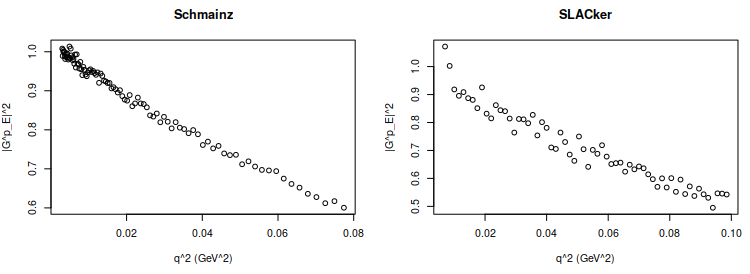
\includegraphics[width=350pt]{raw_data_a.png}
  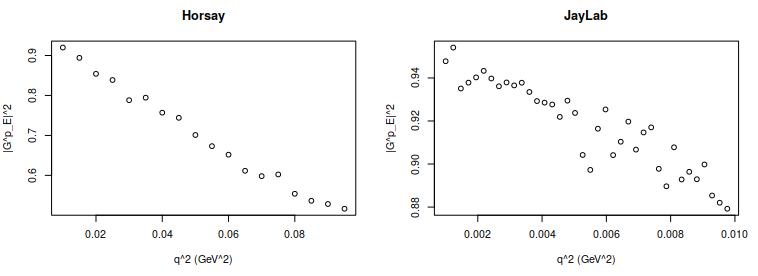
\includegraphics[width=350pt]{raw_data_b.png}
  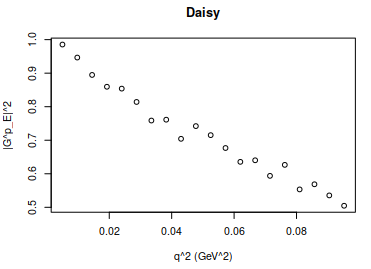
\includegraphics[width=175pt]{raw_data_c.png}
  \caption{Data plotted with R}
\end{figure}

All of the data looks to be in rough agreement.
There will be some difficulty integrating the data together because of the relative size differences.
Particularly between the Schmainz data and the Jaylab data.
Further, inspection, the data could be linear or slightly parabolic, I think adding a fourth order to a polynomial fit would be overkill.
Other models are plausible, but are rather difficult to work with, and could really complicate the analysis.
There may be a periodic wobble in the data, seems most prominent in Schmainz and Daisy, but I might also just be seeing structures that are really just artifacts of random noise.

Throughout the Paper all uncertainties are reported to 1 $\sigma$.


\section{Approach to Fitting}

After a few false starts, I decided that my approach to fitting the data will be to utilize the R data analysis package, and in particular the \texttt{nls()} or non-linear, least squares fitting function on the square of a second order polynomial.
\texttt{nls()} will often struggle finding the proper fit if not given a reasonable guess for starting positions.
To generate the starting position procedurally a linear regression model \texttt{lm()} fit is performed first.
This will the give a line of best fit, of particular interest is a \texttt{y-int} and \texttt{slope}.
These parameters are fed into the \texttt{nls()} model of \texttt{y ~ (A + B * x + C * x * x) ** 2} with \texttt{A} starting at \texttt{y-int}, and \texttt{B} starting at \texttt{y-int}.
The advantage of this model is that it provides a reasonable fit to the data, as seen in the residuals provided below, and the value of \texttt{B}$=\frac{dG_E}{dQ^2}$.
Further \texttt{A*A} is a scaling factor that can be divided out of each data set to renormalise the data permitting use to combine data sets for more advanced analysis.
Other models that were considered included an exponential function, and a 3rd order polynomial. I reasoned that I could essentially treat a polynomial at a Taylor series expansion of an exponential, and since we are interested in a region close to zero, it is just a matter of using a sufficient number of terms. A parabolic function squared was chosen for the fit upon inspection of the residuals of a linear fit, and a cubic function. The parabolic function fit the approximately 2/3 of the data points. 
See the next section for why a periodic function was not attempted to be fit.

\section{Fitting each Experiment}

\begin{figure}[!htb]
  \centering
  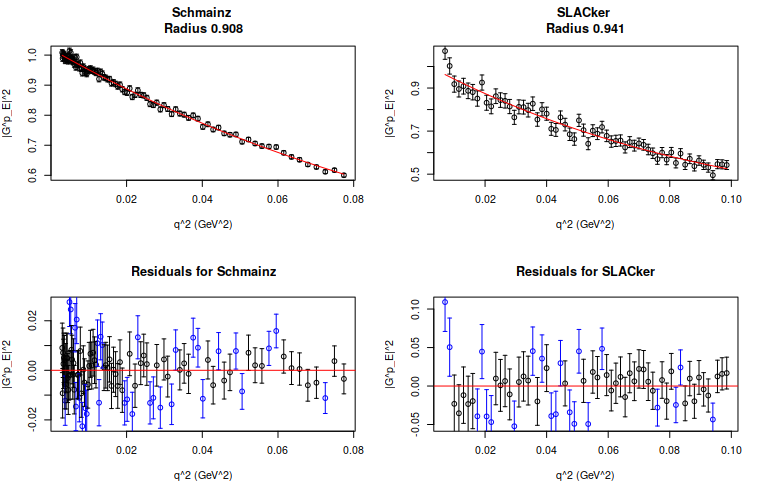
\includegraphics[width=300pt]{fit_data_a.png}
  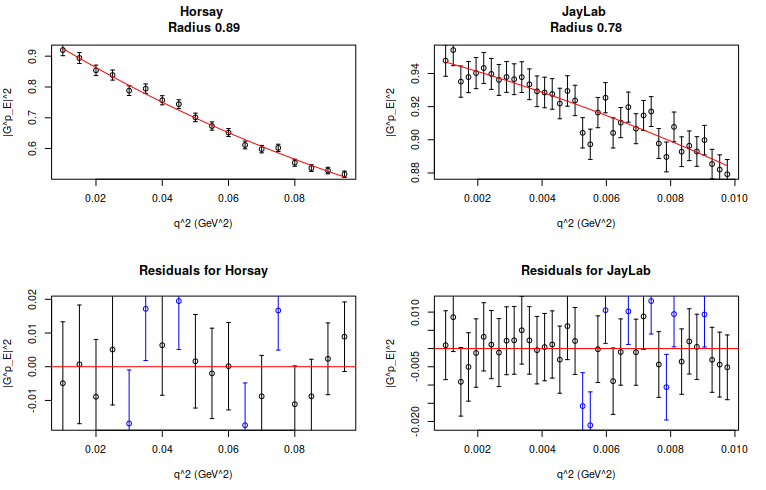
\includegraphics[width=300pt]{fit_data_b.png}
  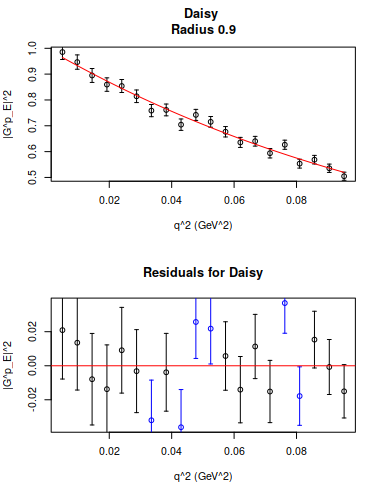
\includegraphics[width=150pt]{fit_data_c.png}
  \caption{Plots after being fit.}
\end{figure}

I drove myself crazy trying to determine if there was a periodicity in the data that I wasn't accounting for in my model. After a few attempts to find periodicity in the data checking for a period I was able to confirm that I was in fact a little bit crazy after I finally plotted the periodicity of $\lvert G_E \rvert^2$ relative to $Q^2$.

\begin{figure}[!htb]
  \centering
  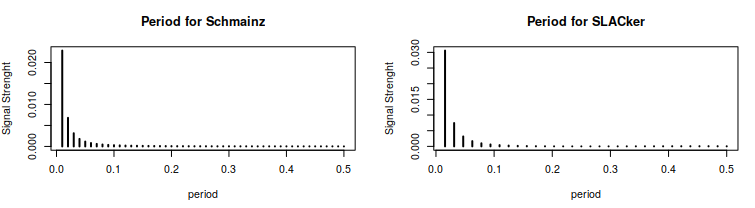
\includegraphics[width=300pt]{period_data_a.png}
  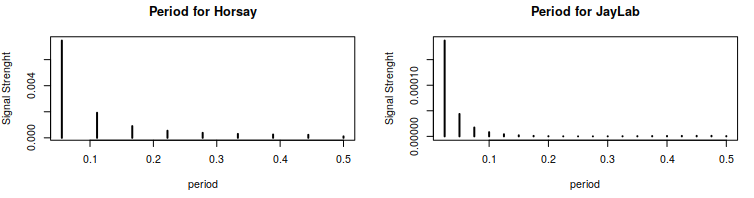
\includegraphics[width=300pt]{period_data_b.png}
  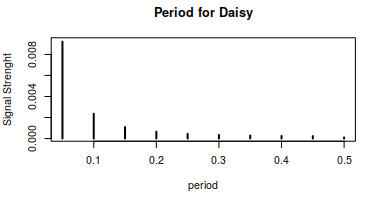
\includegraphics[width=150pt]{period_data_c.png}
  \caption{After seeing the above, I was able to confirm that there was in fact a \texttt{y} value when there was an \texttt{x} value.}
\end{figure}

\pagebreak

\section{Table of Results}

Due to the tricky nature that is error analysis and error propagation of non-linear systems, I choose to do a bootstrap analysis of each of the individual data sets. Each point was randomized by a Gaussian convolution of the reported certainty of the data point, and the systematic error reported by each experiment. Of note, I found the scaling factors to differ from each other from 2\% to 5\% with the data from Jaylab being most suspicious. The bootstrap data set was fit by the same process as the original dataset and 10,000 fits where aggregated and the standard deviation found.

\begin{figure}[!htb]
  \centering
  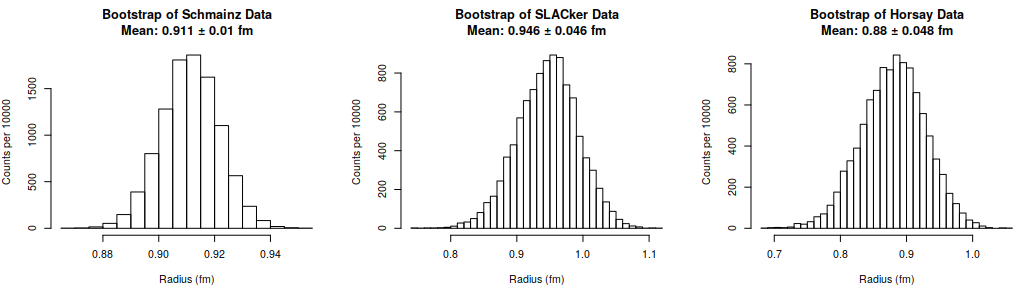
\includegraphics[width=500pt]{exp_hist_data_a.png}
  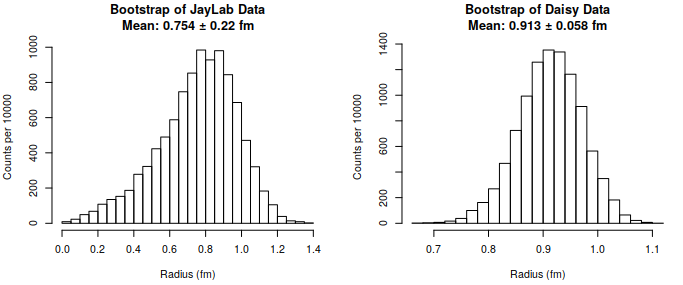
\includegraphics[width=333pt]{exp_hist_data_b.png}
  \caption{These Experiments are in agreement within one $\sigma$}
\end{figure}

\pagebreak

\begin{table}[!htb]
  \centering
  \begin{tabular}{|l|c|c|c|c|c|c|c|}
    \hline
    Experiment      & Schmainz  & SLACker & Horasy  & Jaylab  & Daisy & Average \\\hline
    Proton Rad(fm)  & 0.911     & 0.946   & 0.880   & 0.754   & 0.913 & 0.881   \\\hline
    Standard Dev.   & 0.01      & 0.046   & 0.048   & 0.220   & 0.058 & 0.075   \\\hline
  \end{tabular}
  \caption{For the Average, each experiment was given equal weight.}
\end{table}

\pagebreak

\section{Combined Data}

I handled the combination of the data sets 2 ways.
First I scaled each data set by the inverse of the leading coefficient for each individual data set.
This had the effect of scaling down some and raising others to a rather tight cluster.
I then applied the previously discussed model fitting to the data, to get a first look at the fit.
I then did the bootstrapping method discussed.

This time the boot strap drew a 100 random data points from the entire collection, and applied a Gaussian convolution biased on the reported $\sigma$ of the data point and the 1\% systematic spread reported by each experiment.
(The decision to use the reported numbers in spite of the fact that we know they are off by more than that is accounted for in the next analysis.) 
A histogram of the results was plotted and the standard deviation calculated.

Lastly, in order to account for the fudging that occurred with scaling factors, the raw datasets for all of the experiments where combined with out any scaling factors applied, and then another round of Gaussian convolutions and 10,000 bootstrap analysis was done. This time the data sets were sampled proportional to their size. 


\begin{table}[!htb]
  \centering
  \begin{tabular}{|l|c|c|c|c|c|c|c|}
    \hline
    Technique       & Table Ave   & Normalized Bootstrap  & RAW Bootstrap  \\\hline
    Proton Rad(fm)  & 0.881       & 0.901                 & 0.901          \\\hline
    Standard Dev.   & 0.075       & 0.019                 & 0.019          \\\hline
  \end{tabular}
  \caption{For the Average, each experiment was given equal weight.}
\end{table}

\begin{figure}[!htb]
  \centering
  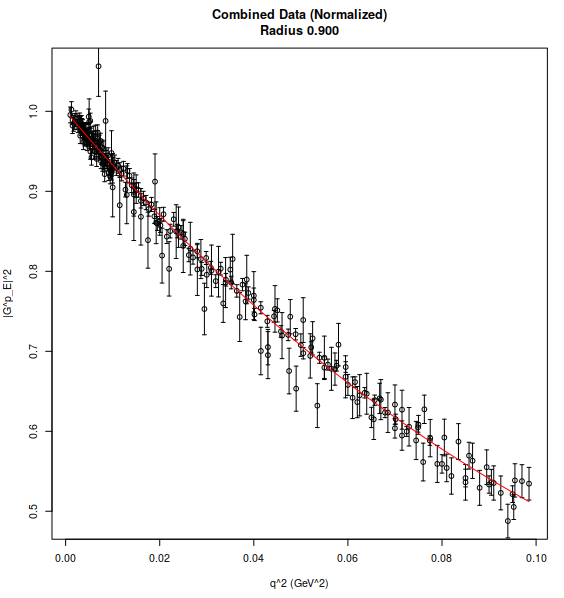
\includegraphics[width=280pt]{combined_data.png}
  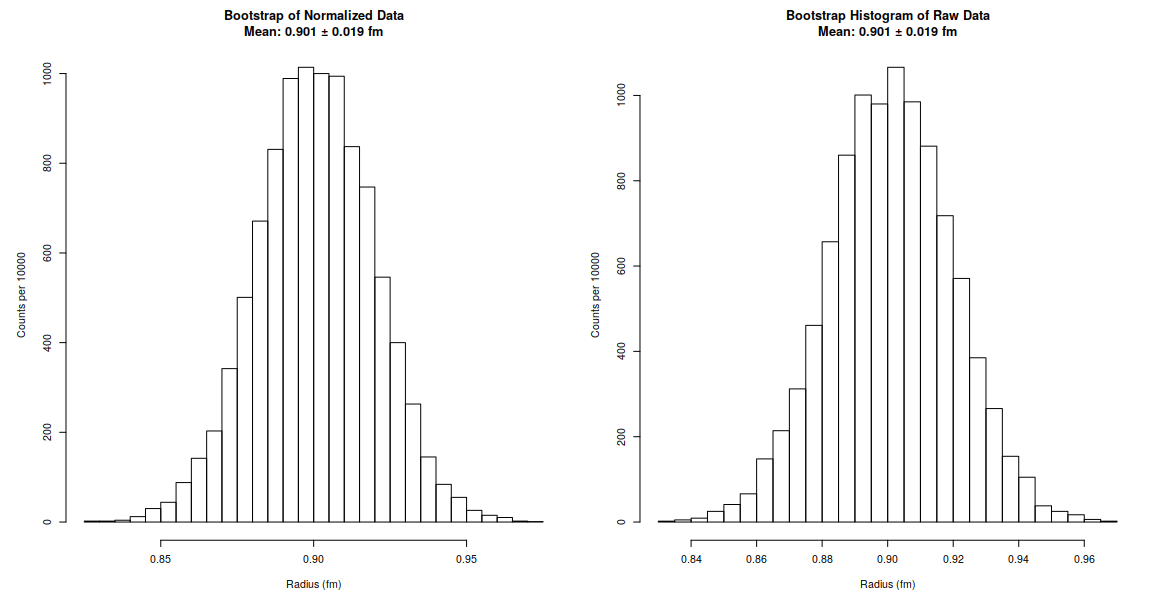
\includegraphics[width=400pt]{hist_data.png}
  \caption{Analysis performed on combined datasets}
\end{figure}

Finally I can report that my best estimation of the Proton Radius is $0.901 \pm 0.019 \mbox{fm}$.


\section{Doing it Better}

One idea worth thinking about is that instead of bootstrapping from the reported points, instead of taking each point and applying a Gaussian convolution, you could extract the curve of best fit, apply a scalar vector to the curve then select points along the curve to generate new points with a Gaussian smearing as well. Then you could draw points equally from each of the experiments, and it would reduce the weight that the Schmainz data has on the analysis.

You might also want to play with some Bayesian techniques starting with the \emph{a priori} radius known, and then using randomly drawn datasets to update the radius. 

I hate to say this, but you can also try tossing out the Jaylab data. Because there are so few points, and the points cover such a short range with such large error bars, the variance in that data set is huge, and it might not be worth holding on to. Especially since they had the largest systematic, and they had the largest uncertainty in their reported data.

One quick edit I could make to my analysis would be to select an experiment at random then draw a point out at random, and then apply the Gaussian convolutions. This would also reduce the weight of Schmainz in the experiment. Then again, Schmainz does seem to be the most reliable of the experiments so\ldots

\end{document}
